\documentclass[11pt]{diazessay} % Font size (can be 10pt, 11pt or 12pt)
% Ecuaciones
\usepackage{amsmath}
% Graficos
\usepackage{tikz}
% Bordes
\usepackage{tcolorbox}
% Bibliografía
\usepackage[
  sorting=none,
  backend=biber,
  style=numeric-comp,
]{biblatex}
\addbibresource{bibliografia.bib}

% Referencias cliqueables
\usepackage{hyperref}
\hypersetup{colorlinks=false}

% Glosario
\usepackage[acronym]{glossaries}
\makeglossaries

% csquotes
\usepackage{csquotes}
%---- Sección de título -----
\title{
  \textbf{Apache Hadoop: Una guía paso a paso
} \\
  {\Large\itshapeUna guía paso a paso
}
} % Titulo y subtitulo

\author{
  \textbf{Ramirez Ulises
} \\
  \textit{Universidad Nacional de Misiones
}\\
  \small\ttulisesrcolina@gmail.com

} % Autor, institución y contacto
\date{} % Date, use \date{} for no date
%---- Sección de título ----

%--------------------------------

\begin{document}
\section*{Historial de Versiones}
Acá se van a detallar los diferentes cambios que se realicen al trabajo luego
de cada entrega a fin de tener una mejor trazabilidad.

En el siguiente repositorio es el que contiene el versionado del trabajo:
\begin{center}
\url{https://github.com/ulisescolina/UC-PYLP/tree/master/Integrador}
\end{center}

\begin{center}
  \begin{tabular}{||p{2cm} p{10cm}||} 
    \hline
    Versión & Cambios \\ [0.5ex] 
    \hline\hline
    1.0.0 & Primer entrega. \\ [0.5ex]
    \hline
    1.0.1 & Segunda entrega (correcciones realizadas por la cátedra):
    \begin{itemize}
        \item Se corrige la forma de redacción en varias partes del documento.
        \item Se corrigen errores ortográficos.
        \item Se corrigen los acrónimos y se agrega la mención de su
          significado en la primer ocurrencia.
    \end{itemize} \\ %[0.5ex]
    \hline
  \end{tabular}
\end{center}
\newpage

 % Notas con respecto al historial de versiones
\maketitle % Print the title section

\renewcommand{\abstractname}{Resumen} % Cambiamos el titulo, en vez de
% decir 'Abstract' va a pasar a decir 'Resumen'
\begin{abstract}
  Este documento es una continuación de lo charlado en el documento introductorio
al modelo \acrlong{mr} (\acrshort{mr})~\cite{ramirez2021}, aquí se procede a la
descripción de cómo configurar un cluster Hadoop para el procesamiento paralelo
y distribuido. En esta instancia la configuración se hará sobre un único nodo.

Algo imporntante a tener en cuenta es que los pasos seguidos para esta configuración
pueden quedar obsoletos ante cambios en distintos paquetes de los cuales
depende el presente tutorial. Se recomienda que ante la incapacidad de poder
realizar una tarea se revisen los canales de distribución oficiales para el
paquete en cuestión.


  \newline\newline
  \textit{\textbf{Palabras clave:} Multiproceso, programación concurrente,
  Procesamiento distribuido, Big Data, MapReduce, Apache Hadoop.
} 
\end{abstract}
\vspace{30pt} % Vertical whitespace between the abstract and first section

%--- Cuerpo -------
\section{Introducción}
\label{sec:introduccion}

El comportamiento por defecto que tiene Hadoop le permite funcionar en entornos
que solamente cuentan con un nodo, a esto se lo llama ``modo local'' (o también
se lo denomina {\it standalone}), un nodo configurado en este modo permitirá la
compilación/ejecución de los mappers y los reducers. A lo largo de las
secciones siguientes se procederá con la configuración de un nodo Hadoop en modo
local.

% una vez se tiene una serie de nodos Hadoop
% configurados en modo standalone, es posible modificar un conjunto de archivos
% de configuración para permitir que estas máquinas interconectadas trabajen de
% manera conjunta.

\section{Big Data}
\label{sec:big_data}

Definir \textit{¿Qué es el big data?} es un trabajo no trivial, anteriormente, se brindó
un concepto que pretendía dar al lector un primer acercamiento al tema, sin
embargo este carece de completitud y especificidad. En
la literatura se demuestra que términos difusos como `grande' hacen aun más
difícil el determinar qué es y qué no es big data, esto supone tener que
definir variables que se van a tomar en cuenta en diferentes disciplinas con el
fin de poder determinar `¿Qué tan grande tiene que ser algo para ser grande?'.

La caracterización principal del big data y por lo tanto la respuesta a la
pregunta anterior se tiene en lo que la literatura llama \textit{las 3
Vs}\footnote{Existen autores que consideran que son
4\textit{V}s\cite{wibowo2019, ghasemaghaei2019}, 5\textit{V}s
\cites{hitzler2013, yin2015}, e incluso autores que
consideran más \textit{V}s~\cite{bonner2017}. Sin embargo, cabe
destacar que estas dos opiniones incluyen las 3\textit{V}s mencionadas
anteriormente.}\cites{bd_ibm, bd_aws, bd_oracle}. Antes de continuar con las \textit{V}s, es conveniente realizar una
aclaración importante: En algunos casos la definición o caracterización aceptada del big data
con las \textit{V}s \textit{no es aplicable}, por ejemplo, en el ámbito de la medicina, Baro {\it et. al}
\cite{baro2015} determinan que la cantidad de datos necesarios para ser grande
se satisface si se cumple que,


\begin{equation} \label{eq-baro2015-1}%
  \log_{10}(n * p) \geq 7 \\
\end{equation}

En donde se tiene que,

\begin{tabular}{l l}
$n$ & Cantidad de \textit{individuos estadísticos}\\
$p$ & Cantidad de variables a ser analizadas \\
    & dentro del \gls{dataset}\\
\end{tabular}

% Siendo $n$ la cantidad de \textit{individuos estadísticos}
% y $p$ la cantidad de variables a ser analizadas dentro del \gls{dataset}
% compuesto por un conjunto de artículos.


En este caso específico analiza el significado de ¿Qué es ser big data? para un
área en particular, \textit{la medicina}\footnote{cabe destacar que no es posible asumir que este
análisis llevado a cabo por los autores es trasladable a todas las
disciplinas}, aquí se busca enfocar y delimitar el concepto de
grande al área de la salud. El motivo principal detrás de esto es que luego de
estudiar los diferentes casos (entendiendo como \textit{casos} las
publicaciones en revistas científicas orientadas exclusivamente a la medicina)%a la hora de trabajar con los datos dentro de
en un ambiente orientado a la salud, no se satisfacen los criterios de
masividad\footnote{Comparado con la cantidad de consultas que recibe Google, la
cantidad de reseñas escritas en Amazon, la cantidad de comentarios que se
publican en Twitter, etc.}, pero aún así existe en el corpus material acerca
del big data asociado a la medicina, por lo que se hace útil poseer una
definición mas ajustada a dicha disciplina.


\subsection{Volúmen}
\label{ssec:volumen}

El volúmen hace referencia a la cantidad de datos dentro de un \gls{dataset}\cites{ghasemaghaei2019,
ghasemaghaei2021}, considerado por algunos autores como la característica que
brinda los mayores desafíos para el tratamiento con el big data\cite{che2013}.

Se habla de cantidad, y nuevamente se tiene esta idea de \textit{¿Qué tantos datos hacen
falta para tener un volúmen lo suficientemente masivo como para ser considerado
grande?}

Hacia el 2010, el mundo había creado 1\acrshort{zb}\footnote{NOTA: 1\acrshort{zb} equivale a $1 \times
10^{9}$ terabytes, es decir 1000000000\acrshort{tb}.} de datos, se menciona
esto para tener
una idea aproximada de la cantidad de datos manejados hace DIEZ AÑOS ATRAS! (una
eternidad en el mundo de las tecnologías de la
información),  y se estimaba que para el 2020 el mundo habría creado 40\acrshort{zb}\cite{lam2017}, 
sin embargo, para 2018 ya se tenían 33\acrshort{zb}, lo cual llevó al
\acrlong{idc} (\acrshort{idc}) a 
realizar nuevas consideraciones y se terminó estimando
que para 2025 se tendrían 175\acrshort{zb}\cite{forbes2020}. Es decir,
que en el tramo de 15 años, lo que se consideraba inconmensurable al inicio
multiplicaría su tamaño por 175. Hablar de estas magnitudes se
va naturalizando a medida que pasa el tiempo, ya en el 2013 se iba haciendo
cotidiano hablar de Petabytes (\acrshort{pb}) de cara al uso de
Exabytes (\acrshort{eb})\cite{che2013}. 


\subsection{Variedad}
\label{ssec:variedad}

Esta es otra de las características principales dentro del big data,
y hace referencia a la variedad de datos que conforman un \gls{dataset}. Este
fenómeno tiene lugar por el simple hecho de que existen casi ilimitadas fuentes
que pueden contribuir a un \gls{dataset}, el cual puede estar compuesto por
diferentes tipos y formas de representaciones\cite{che2013} lo cual hace al big
data grande y estos pueden ser resumidos en estructurados, semi-estructurados y
no-estructurados\cite{sagiroglu2013}.

Los datos estructurados y los semi estructurados caben en los Sistemas de Administración de Bases de
Datos (\acrshort{dbms}) y/o Data-Warehouses (\acrshort{dw}), acá se mencionan
los semi estructurados porque estos estan compuestos por archivos tales como
XML, en donde se tienen etiquetas para separar diferentes elementos de datos.
En cuanto a los datos no estructurados se puede mencionar a la web como una
fuente importante de los mismos, un ejemplo primordial aquí es el denominado
\gls{clickstream}\cites{russom2011, albert2010-c05}, aunque menciones
honorables van además para los mensajes de textos que se obtienen de las
compañias de celulares, datos generados por sensores en dispositivos
\acrshort{iot}, etc.

\subsection{Velocidad} \label{ssec:velocidad}

En la introducción se hizo mención de la utilidad de herramientas para
análisis de datos, más específicamente, se habló de Almacenes de Datos o 
\acrlong{dw}/\acrlong{edw} (\acrshort{dw}/\acrshort{edw}), y su contribución
superlativa a la Inteligencia de Negocios (\acrshort{bi}) mencionada en la
Sección \ref{sec:introduccion}.

Este sistema utilizado en \acrshort{bi} es una respuesta para múltiples
desafíos que se tienen dentro de una organización\cite{datalytics2}, en este
documento se hace énfasis concretamente en uno de los motivos, el 
\textit{para dar soporte a las desiciones que se toman a nivel estratégico}.
Para lograr ese soporte, la organización 
sigue una metodología que le va a permitir aplicar estas herramientas
analiticas con el fín de extraer el valor de los datos. La gente de
Datalytics\footnote{https://www.datalytics.com/}, menciona a lo largo de varias
charlas que componen el ciclo de ``DataSchool'', la importancia de estas
arquitecturas clásicas, sin embargo, el acercamiento clásico a la creciente
cantidad de datos brinda más desafíos, particularmente el que más resuena en el
contexto de este documento es el hecho de que esta arquitectura tradicional es 
\textit{lenta para reaccionar}\cite{datalytics3}.

El concepto de velocidad es esto, y es tan importante como los que se hablaron
anteriormente. La velocidad a la que se pueda realizar un análisis concreto y
tomar decisiones basadas en los resultados es clave. El análisis de un
fragmento de información acerca de la competencia, datos estadísticos realizados
por algún organismo ajeno a la organización que tiene una periodicidad anual
(ej: \acrshort{indec}), etc. posee una gran potencialidad, sin embargo, si no
se analiza oportunamente, el valor que pueda existir en esa información se
pierde.




% Alguna conclusión probablemente para el tema de BD

\section{Procesamiento Paralelo}
\label{sec:procesamiento_paralelo}
%Pequeña introduccion de que es el procesamiento paralelo
% - Explicar que existen tres caminos de paralelizacion, aunque la tercera
%   la que está basada en redes de neuronas, es un sistema que difiere al que
%   se viene viendo.

Diversos autores\cite{moldovan93, trobec2018} describen en profundidad diferentes modelos que
extienden a la arquitectura tradicional de Von Neumann para lograr
paralelización\footnote{No es el objetivo de este documento dar una descripción minuciosa de los
diferentes modelos teóricos de paralelización.}. Esta se logra mediante la separación de una tarea $T$, en subtareas
$T_{1}, T_{2}, \ldots , T_{n}$ (Diferentes autores adoptan este concepto con el
término de \textit{\gls{pipelining}}~\cite{hyde98, trobec2018}). Luego para lograr el cometido, 
más de una de las $T_{n}$ tareas debe realizarse al mismo tiempo, sin malinterpretar la
realización de una tarea de manera muy velóz con realizarla al mismo tiempo que
otras~\cite{hyde98}.

Las diferentes soluciones para procesamiento paralelo se desenvolvieron hasta
llegar a presentar uno de los siguientes tres tipos de
paralelismo\cite{trobec2018}:

\begin{itemize}
\item Los {\bf Sistemas de Memoria Compartida} que se componen de múltiples unidades de procesamiento
unidas a una memoria.
\item Los {\bf Sistemas Distribuidos} que se componen de equipos con sus propias unidades de procesamiento
y memoria, comunicados a traves de una conexión de red de alta velocidad. Este
es el caso que nos compete en este documento y es tratado en la Sección
\ref{sec:procesamiento_distribuido}.
\item Las {\bf Unidades de Procesamiento Gráfico} utilizadas como co-procesadores por su
capacidad de paralelizar grandes cantidades de operaciones.
\end{itemize}

Diferentes enfoques existen a la hora de aplicar el \gls{pipelining} mencionado
anteriormente, y estos no son recientes sino que datan desde la década de 1990.
Con el pasar del tiempo se fueron creando más enfoques y especializando los
casos generales que se tenían en un principio. Ejemplo de algunas
especializaciones son los enfoques que se ven en la cátedra de Paradigmas y Lenguajes 
de Programación\cite{pylp1}, en donde se denomina a este problema
\textit{Descomposicion}, y de ahí surgen las diferentes especializaciones:
Dominio, Funcion, Recursiva, Mixta.

Para este documento solamente se tienen en cuenta dos de las 3 que se 
proponen por Fountain~\cite{fountain1994}: Paralelización de Datos y
Paralelización de Funciones.

La paralelización de datos y la paralelización de funciones puede encontrarse 
en diferentes niveles de la arquitectura
del computador, algunos ejemplos van desde, el procesador como lo describe
Hyde~\cite{fountain1994}, pasando por el compilador~\cite{clark1997}, llegando
a la aplicación~\cite{wolters1995}, etc. Este 
documento cubre únicamente a casos que son aplicados a nivel de aplicación.

\subsection{Paralelización de Datos}
\label{ssec:paralelizacion_de_datos}

\begin{tcolorbox}
La idea principal detrás de este enfoque a la hora de aplicar el {\it pipelining}
consiste en que un programa secuencial puede ser transformado a un
programa paralelo, realizando ejecuciones de copias idénticas de dicho programa como
tareas separadas, a las cuales se les brinda simplemente parte de los datos
iniciales~\cite{haveraaen2000}.
\end{tcolorbox}

En la figura \ref{fig:sin_paralelizacion_datos} se presenta una aplicación que
está corriendo sobre un núcleo aleatorio en un ordenador. En este ejemplo no se tiene
presente la paralelización, $D$ representa los datos sobre los cuales está
trabajando la \textit{Aplicación}.

\begin{figure}[h]
  \centering
  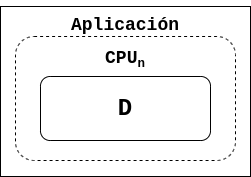
\includegraphics[width=0.3\linewidth]{figuras/procesamiento_paralelo_sin_paralelizacion_datos.png}
  \caption{Aplicación sin paralelización}
  \label{fig:sin_paralelizacion_datos}
\end{figure}

En la figura \ref{fig:con_paralelizacion_datos} se presenta la misma
aplicación (esta vez se la denomina \textit{app}). En este ejemplo
los datos representados por $D$ anteriomente, se
dividien en $D_{n}$ secciones más pequeñas que son distribuidas a distintos
núcleos de procesamiento \footnote{en el ejemplo se utilizan 4, aunque pueden ser más
núcleos dentro de un procesador}. Una copia idéntica de la aplicación (Figura
\ref{fig:sin_paralelizacion_datos}) se encuentra corriendo en cada uno de los
cuatro núcleos del ordenador, cada una de estas copias idénticas se
encuentra trabajando con datos distintos (ya que a cada una de las copias le
toca una sección $D_{n}$ diferente).

\begin{figure}[h]
  \centering
  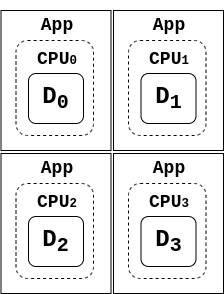
\includegraphics[width=0.3\linewidth]{figuras/procesamiento_paralelo_con_paralelizacion_datos.png}
  \caption{Aplicación con paralelización de datos}
  \label{fig:con_paralelizacion_datos}
\end{figure}

Una interpretación alternativa se puede ver en la figura
\ref{fig:con_paralelizacion_datos_alt}, este gráfíco se puede leer como ``Una
aplicación que se encuentra corriendo sobre distintos nucleos, con distintos
fragmentos de los datos originales''

\begin{figure}[h]
  \centering
  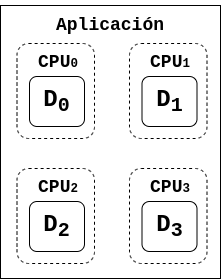
\includegraphics[width=0.3\linewidth]{figuras/procesamiento_paralelo_con_paralelizacion_datos_alt.png}
  \caption{Aplicación con paralelización de datos - Representación alternativa}
  \label{fig:con_paralelizacion_datos_alt}
\end{figure}


En la bibliografía existen implementaciones en diferentes sub áreas de las Ciencias de la
Computación con este enfoque presente, el procesamiento de
imágenes~\cite{pang2009}, el manejo de bases de
datos~\cite{zakharov2019} y la inteligencia artificial~\cite{hajj2015} por
nombrar algunos ejemplos. 

Para un ejemplo simple y concreto se propone lo siguiente: 

\begin{tcolorbox} \label{ej:1} 
  Se presenta la tarea de encontrar el valor mínimo dentro de un arreglo 
  $A = [a_{0}, a_{1}, \ldots , a_{n-2}, a_{n-1}]$.
\end{tcolorbox}

Se puede proceder sin aplicar paralelización de datos, y realizar una
aplicación que recorra los $n$ elementos del arreglo, realice las
comparaciones necesarias y devuelva el valor mínimo, o se puede
optar por la opción con paralelización de datos, una solución con este enfoque 
será fraccionar el arreglo con $A$ en, por ejemplo, 2 partes $A_{1}$ y
$A_{2}$. Luego se procede a distribuir estas dos partes $A_{1}$ y
$A_{2}$ a diferentes instancias de la aplicación que calcula el mínimo, 
de esta manera se tendrán dos núcleos de procesamiento que trabajarán en un
problema de menor tamaño (ya que
cada uno va a trabajar únicamente con el 50\% de los datos), y al final
solamente hará falta realizar una comparación entre los mínimos que
encuentren las dos instancias de la aplicación.

Cabe destacar que algunos problemas pueden surgir a la hora de particionar
datos si esto se hace sin nignun análisis, un ejemplo de esto puede ser
considerado en el escenario en donde ocurre
la división de una imagen en partes más pequeñas para su análisis en forma
paralela~\cite{oshitani1999}. También se hace presente la limitación que impone
la ley de Amdhal\footnote{``El incremento máximo de velocidad (la cantidad máxima de
procesadores que pueden ser utilizados de manera efectiva) es la inversa de la
fracción de tiempo que la tarea toma para finalizar en un solo
hilo'' \cite{rodgers1985}}.
% \begin{figure}[h]
  \centering
  \label{fig:paralelizacion_datos}
  \resizebox{!}{5cm}{%
    \begin{tikzpicture}
      % Dato
      \draw (0,4.75) rectangle (5,8.75) node[midway,blue]{\texttt{Datos}: $1,2,3,4,5,6,7,8,9,10$};

      % Datos
      \draw (9, 10) rectangle(10.5,11.5) node[midway,blue]{$1,2$};
      \draw (9, 8) rectangle (10.5,9.5) node[midway,blue]{$3,4$};
      \draw (9, 6) rectangle (10.5,7.5) node[midway,blue]{$5,6$};
      \draw (9, 4) rectangle (10.5,5.5) node[midway,blue]{$7, 8$};
      \draw (9, 2) rectangle (10.5,3.5) node[midway,blue]{$9, 10$};
    \end{tikzpicture}
  }
  \caption{Concepto paralelización de datos}
\end{figure}


\subsection{Paralelización de Funciones}
\label{ssec:paralelizacion_de_funciones}

\begin{tcolorbox}
  Este enfoque a la paralelización toma otro camino a la hora de aplicar el
  \textit{pipelining}, este acercamiento
  no fracciona los datos sino que transforma la tarea a un gráfo de 
  dependencias en donde cada nodo corresponde a una operación a ser realizada
  para cumplir la tarea. Y lo que trata de hacer es ejecutar la mayor
  cantidad de tareas al mismo tiempo~\cites{meng2013, liu2019, zhou2020,
  lin2021}.
\end{tcolorbox}

Esta idea de distribuir los datos a diferentes unidades funcionales que se
encarguen de realizar una tarea sobre los datos mencionados se presenta en la
figura \ref{fig:con_paralelizacion_funciones}.

% En la figura \ref{fig:con_paralelizacion_datos} se presenta la misma
% aplicación (esta vez se la denomina \textit{app}). En este ejemplo
% los datos representados por $D$ anteriomente, se
% dividien en $D_{n}$ secciones más pequeñas que son distribuidas a distintos
% núcleos de procesamiento \footnote{en el ejemplo se utilizan 4, aunque pueden ser más
% núcleos dentro de un procesador}. Una copia idéntica de la aplicación (Figura
% \ref{fig:sin_paralelizacion_datos}) se encuentra corriendo en cada uno de los
% cuatro núcleos del ordenador, cada una de estas copias idénticas se
% encuentra trabajando con datos distintos (ya que a cada una de las copias le
% toca una sección $D_{n}$ diferente).

Aquí se puede observar que lo que se subdivide no son los datos, sino que lo que
se está subdividiendo es la funcionalidad que compone a la tarea $T$, aquí cada
$o_{n}$ es una operación claramente delimitada dentro de la aplicación, y $D$
representa a los datos con los que se va a trabajar.

\begin{figure}[h]
  \centering
  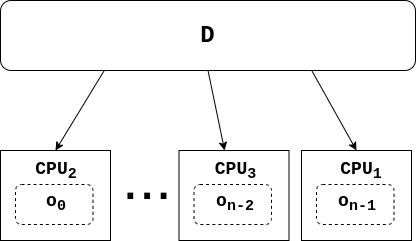
\includegraphics[width=0.65\linewidth]{figuras/procesamiento_paralelo_con_paralelizacion_func.png}
  \caption{Aplicación con paralelización de funciones}
  \label{fig:con_paralelizacion_funciones}
\end{figure}


Un ejemplo concreto para este enfoque se presenta a continuación:

\begin{tcolorbox}
  Dada una imagen, se presenta la tarea de determinar si en dicha imagen se
  encuentra presente algún rostro, vehículo, gato o planta.
\end{tcolorbox}

Por lo que se puede decir que la tarea $T$ se compone de la siguiente manera

\begin{equation} \label{eq-tareas-nodos}%
  T = [o_{0}, o_{1}, o_{2}, o_{3}]
\end{equation}

En donde se tiene que,

\begin{tabular}{l   l}
$o_{0}$ & Buscar rostro \\
$o_{1}$ & Buscar vehículo \\
$o_{2}$ & Buscar planta \\
$o_{3}$ & Buscar gato\\
\end{tabular}

\vspace{1cm}

Cada $o_{n}$ en la ecuación \ref{eq-tareas-nodos} representa un nodo del gráfo
de mencionado anteriormente. Ahora toca analizar y determinar
cuales de las $o_{n}$ operaciones se pueden realizar al mismo tiempo.

Una cuestion esencial en este ejemplo es identificar el hecho de que ninguna
operación $o_{n}$ depende de alguna operación.
% $o_{m}$ $\forall m, n \in
% \mathbb{N}| 0 \leq m, n \leq 3$
Esto es visible a la hora de realizar diversas preguntas con
respecto al contexto, 
\begin{itemize}
    \item ¿Es necesario determinar si existe o no un rostro para poder iniciar
      el análisis y determinar si la imagen contiene un vehiculo, gato o
      planta? No, entonces, {\it Buscar rostro} es independiente a las demás
      operaciones.
    \item ¿Es necesario determinar si existe un vehiculo en la imagen para
      poder iniciar el análisis y determinar si la imagen contiene un rostro,
      gato o planta? No, entonces, {\it Buscar vehículo} es independiente a las
      demás operaciones.
\end{itemize}

El análisis anterior debe continuar hasta que se analicen las $o_{n}$
operaciones. Habrán veces en donde dos o más operaciones no podrán ser ejecutadas de
manera paralela, esto puede darse porque una (también pueden ser varias) de ellas 
depende de los resultados que se obtengan de otra u otras operaciones.

En el caso del ejemplo para la sección, esta apreciación y el análisis que se
realizó permite definir que todas las operaciones que componen a la tarea $T$
se pueden ejecutar de manera paralela por el mismo dato.

\section{Procesamiento Distribuido}
\label{sec:procesamiento_distribuido}

Este tiene muchas similitudes con los sistemas de Procesamiento Paralelo, es
más, es válido decir que los Sistemas Paralelos y los Sistemas Distribuidos son
un entrelazamiento de redes, que tienen la caracteristica de ser
continuas\footnote{
o un \gls{continuum} de redes.
\url{https://dictionary.cambridge.org/es/diccionario/ingles/continuum}}, lo que
significa que el parámetro que determina si el sistema es distribuido es el promedio de
distancias entre los nodos de procesamiento~\cite{hyde98}. El desafío que
propone Hyde, y también diferencia a los dos sistemas es el de poder determinar el
estado exacto de todo el sistema. Este es un desafío no-trivial, ya que dicho
estado no puede ser computado
instantaneamente por el hecho de que cada operación dentro de la red podría
requerir travesías por la misma.

%--- Fin Cuerpo ---

%- Bibliografía -
\clearpage
% \printbibheading
% \printbibliography[type=article, heading=subbibliography, title={Articulos}]
% \printbibliography[type=book, heading=subbibliography, title={Libros}]
% \printbibliography[type=online, heading=subbibliography, title={Recursos en
% línea}]
\printbibliography
%----------------

%--- Glosario ---
% \clearpage
\clearpage
% Terminos
\newglossaryentry{wearables}{
  name=wearables,
  description={\textit{Vestible}, En el contexto de la tecnología, hace referencia a un
  dispositivo que se pueda \textit{vestir}. Ej: relojes inteligentes}
  }

\newglossaryentry{dataset}{
  name=dataset,
  plural=datasets,
  description={\textit{Conjunto de datos}, sobre los cuales se realizan experimentos.
  Las conclusiones que los investigadores definan sobre un cierto tema, se da
  mediante los experimentos realizados sobre uno o más conjuntos de datos}
  }

\newglossaryentry{clickstream}{
  name=clickstream,
  description={\textit{Flujo de clicks}, es una bitacora detallada de como los usuarios
  navegan una página web al realizar una tarea}
  }

\newglossaryentry{continuum}{
  name=continuum,
  description={\textit{Continuo}, algo que cambia gradualmente o en pequeños
  incrementos sin ningún pico evidente}
  }

\newglossaryentry{pipelining}{
  name=pipelining,
  description={En Ciencias de la Computación, este hace
  referencia a una organización en la cual pasos sucesivos de una secuencias de
  instrucciones son ejecutadas por diferentes módulos, esto para que otra
  instrucción pueda iniciar antes que una instrucción anterior finalice}
  }

\newglossaryentry{framework}{
  name=framework,
  plural=frameworks,
  description={\textit{Marco de trabajo}, es un conjunto estandarizado de 
  conceptos, prácticas y criterios para enfocar un tipo de problemática particular
  que sirve como referencia, para enfrentar y resolver nuevos problemas de índole 
  similar}
  }

\newglossaryentry{cluster}{
  name=cluster,
  plural=clusters, 
  description={\textit{Grupo} o también llamado \textit{Granja de servidores},
  es un término que se aplica a los sistemas distribuidos y hace referencia a 
  un conjunto de máquinas interconectadas por una red de alta velocidad}
  }

\newglossaryentry{heartbeat}{
  name=heartbeat,
  plural=heartbeats, 
  description={\textit{Latido}, es una señal periódica generada por
  software para indicar que el funcionamiento está funcionando adecuadamente, o
  para la sincronización con otras partes del sistema}
  }

% Siglas
\newacronym{iot}{IoT}{Internet of Things}
\newacronym{bi}{BI}{Business Intelligence}
\newacronym{dbms}{DBMS}{Data Base Management Systems}
\newacronym{dw}{DW}{Data Warehouse}
\newacronym{edw}{EDW}{Enterprise Data Warehouse}
\newacronym{eb}{EB}{Exabyte}
\newacronym{gb}{GB}{Gibabyte}
\newacronym{gfs}{GFS}{The Google File System}
\newacronym{hdfs}{HDFS}{Hadoop File System}
\newacronym{indec}{INDEC}{Instituto Nacional De Estadística y Censos}
\newacronym{jar}{JAR}{Java Archive Format}
\newacronym{jvm}{JVM}{Java Virtual Machine}
\newacronym{mr}{MR}{MapReduce}
\newacronym{tb}{TB}{Terabyte}
\newacronym{pb}{PB}{Petabyte}
\newacronym{pram}{PRAM}{Parallel Random-Acces Machine}
\newacronym{zb}{ZB}{Zettabyte}


\printglossary[type=\acronymtype] % Si no esta este no imprime los acrónimos
\printglossary % Si no esta este con el anterior no imprime los términos del glosario
%----------------

\clearpage
\section*{Anexo: Terabytes $\Rightarrow$ Petabytes $\Rightarrow$ Exabytes $\Rightarrow$ Zettabytes}
\label{sec:petabytes_a_zettabytes}

A veces, tratar magnitudes tan extremas no permite transmitir de manera
comprensible lo masivo o lo ínfimo de tales magnitudes,
esto es frecuentemente el caso al hablar de cantidad de
datos tales como los Terabytes, Petabytes, Exabytes o Zettabytes.

Si el lector es una persona que esta familiarizada con los medios de almacenamiento
y su tamaño, resulta sencilla la explicación de que un Terabyte es mayor que
un Gigabyte, esto puede deberse a que el Gigabyte es una unidad que se utiliza
cotidianamente, por ejemplo, el tamaño de los pendrives, la memoria del celular,
el tamaño de discos en ordenadores, etc. Sin embargo, esta explicación puede
volverse un desafío si se intenta realizar la explicación a una persona que no
posee conocimiento alguno acerca de este tema, o incluso si la capacidad que se
intenta explicar es lo suficientemente masiva como por ejemplo los mencionados
Zettabytes (\acrshort{zb}).

En este anexo, se propone un ejemplo para que el lector (independientemente de
su nivel en el uso de tecnología) se familiarice y tenga una mejor
concepción la masividad a la hora de hablar del salto desde Gigabytes a
Zettabytes. En este ejemplo no se van a utilizar
conceptos de las ciencias de la computación, se va a tratar 
con segundos, minutos, horas, días y años, conceptos que se puede asumir son
familiares y que son asimilados por todos los lectores.

Para iniciar, podemos partir desde el Gigabyte (\acrshort{gb}), y podemos decir
que un \acrshort{gb} en este anexo va a contar como $1$ seg. Partiendo de esa
premisa, el siguiente cuadro posee las equivalencias en segundos para cada unidad
mencionada anteriormente, utilizando, minutos, horas, días y años a medida que
se haga necesario.

\begin{table}[h]
  \centering
  \begin{tabular}{||r r c c c c||} 
   \hline
    Unidad & Segundo(s) & Minutos & Horas & Días & Años \\ [0.5ex] 
   \hline\hline
   \acrlong{gb} (\acrshort{gb}) & 1 & --- & --- & --- & --- \\ 
   \hline
   \acrlong{tb} (\acrshort{tb}) & 1024 & 17 & --- & --- & --- \\
   \hline
   \acrlong{pb} (\acrshort{pb}) & 1048576 & --- & 291 & 12 & --- \\
   \hline
   \acrlong{eb} (\acrshort{eb}) & 1073741824 & --- & --- & 12428 & 34 \\
   \hline
   \acrlong{zb} (\acrshort{zb}) & 1099511627776 & --- & --- & --- & 34865 \\ [1ex] 
   \hline
  \end{tabular}
  \\
  \label{unidades:gb_a_zb}
  \caption{Escala de unidades con su equivalencia temporal}
\end{table}

Es decir, si se compara a el \acrlong{gb} con el \acrlong{zb}, se ve la
masividad de la que se está hablando, y se hace palpable al extrapolar estos
valores tan grandes a un concepto cotidiano como el tiempo. 1\acrshort{gb} = 1
segundo y tenemos que 1\acrshort{zb} = 34865 {\bf AÑOS}. Se puede quere acortar
la diferencia y comparar dos unidades más cercanas como por ejemplo el
\acrlong{pb} y el \acrlong{zb}. Pero incluso con este acercamiento la
diferencia es extrema ya que se tiene que 1\acrshort{pb} = 12 Días mientras que
1\acrshort{zb} es 34865 {\bf Años}.


\end{document}
